Given is the continuous signal:
{
	\setlength{\abovedisplayskip}{0pt}
	\setlength{\belowdisplayskip}{6pt}
	\setlength{\abovedisplayshortskip}{0pt}
	\setlength{\belowdisplayshortskip}{0pt}
	\begin{align*}
		s(t) = \cos\left[{\omega_0\cdot\left(t-\tau_0\right)+\theta_0}\right]
	\end{align*}
}
\renewcommand{\labelenumi}{\alph{enumi})}

\newenvironment{nscenter}
{\parskip=0pt\par\nopagebreak\centering}
{\par\noindent\ignorespacesafterend}
\begin{enumerate}
	\item
		Calculation of the frequency and period duration, as well as representation of the signal curves for the cases:
		\begin{nscenter}
			\begin{tabular}{c|lll}
				& $\omega_0$ & $\tau_0$ & $\theta_0$ \\
				\hline
				1 & $\pi/3$ & $0$ & $2\pi$ \\
				2 & $3\pi/4$ & $1/2$ & $\pi/{4}$ \\
				3 & $3/4$ & $1/2$ & $1/4$ \\
			\end{tabular}
		\end{nscenter}
		
		\subsubsection{General information}
		The frequency $f$, defined as the number of oscillations within a unit of time, given in $\si{\Hz} = 1\fracslash\si{\s}$. In general, the frequency is described by the quotient of wave speed $c$ and wavelength $\lambda$. Alternatively, it can also be derived using the circular frequency $\omega$. This is based on the assumption that a complete oscillation on a circle of $2\pi$ requires exactly one frequency.
		{
			\setlength{\abovedisplayskip}{0pt}
			\setlength{\belowdisplayskip}{6pt}
			\setlength{\abovedisplayshortskip}{0pt}
			\setlength{\belowdisplayshortskip}{0pt}
			\begin{align*}
				\omega = 2\pi{f} \rightarrow f = \frac{\omega}{2\pi}
			\end{align*}
		}%
		The period duration $T$ indicates the time required to complete a full oscillation. From this follows formally
		{
			\setlength{\abovedisplayskip}{0pt}
			\setlength{\belowdisplayskip}{6pt}
			\setlength{\abovedisplayshortskip}{0pt}
			\setlength{\belowdisplayshortskip}{0pt}
			\begin{align*}
				T = \frac{1}{f}
			\end{align*}
		}
		
		\subsubsection{Solution}
		{
			\setlength{\abovedisplayskip}{0pt}
			\setlength{\belowdisplayskip}{6pt}
			\setlength{\abovedisplayshortskip}{0pt}
			\setlength{\belowdisplayshortskip}{0pt}
			\sisetup{parse-numbers=false}
			\begin{flalign*}
				&f_1 = \frac{\frac{\pi}{3}}{2\pi} = \frac{\pi}{3\cdot{2}\pi} = \SI{\frac{1}{6}}{\Hz} &
				&T_1 = \frac{1}{\frac{1}{6}} = \SI{\frac{6}{1}}{\s} = \SI{6}{\s} & \\
				%
				&f_2 = \frac{\frac{3\pi}{4}}{2\pi} = \frac{3\pi}{{4}\cdot2\pi} = \SI{\frac{3}{8}}{\Hz} & 
				&T_2 = \frac{1}{\frac{3}{8}} =  \SI{\frac{8}{3}}{\s} \approx \SI{2,6\overline{6}}{\s} & \\
				%
				&f_3 = \frac{\frac{3}{4}}{2\pi} = \frac{3}{4\cdot2\pi} = \SI{\frac{3}{8\pi}}{\Hz} \approx \SI{0,12}{\Hz} & 
				&T_3 = \frac{1}{\frac{3}{8\pi}} = \SI{\frac{8\pi}{3}}{\s} \approx \SI{8,38}{\s} & 
			\end{flalign*}
			
			Signal curves\newline
			The signal curves $s_n(t)$, are drawn in the interval $0 \leq t \leq 4\pi$.
			
			\pgfplotsset{
				axis411a/.style={
					xlabel=$t$,
					x label style={at={(current axis.right of origin)},	anchor=east, right=1mm},
					y label style={at={(current axis.above origin)}, anchor=south }
				},
			}
			
			\begin{tikzpicture}
				\begin{groupplot}
					[
						group style={
							group size=1 by 3,
							xlabels at=edge bottom,
							ylabels at=edge left,
							horizontal sep=0.2\textwidth, group name=plots,
						},
						width=\linewidth,
						height=4cm,
						ylabel=$s$,
						ymin=-1.1, ymax=1.1,
						ytick={-1,-0.5,0,0.5,1},
						axis x line=middle,
						axis y line=center,
						tick align=outside,
						hide obscured y ticks=false,
						grid=both,
						grid style={line width=.1pt, draw=gray!10},
						major grid style={line width=.2pt,draw=gray!30},
						ytick distance = 1,
						xtick={-2*pi, -(3*pi)/2, -pi, -pi/2, pi/2, pi, (3*pi)/2, 2*pi, (5*pi)/2, 3*pi, (7*pi)/2, 4*pi},
						xticklabels={$-2\pi$, $-\frac{3\pi}{2}$, $-\pi$, $-\frac{\pi}{2}$, $\frac{\pi}{2}$, $\pi$, $\frac{3\pi}{2}$, $2\pi$, $\frac{5\pi}{2}$, $3\pi$, $\frac{7\pi}{2}$, $4\pi$ },
						domain=0:4*pi+0.2
					]
					\nextgroupplot[title=$s_1(t)$, axis411a]
					\addplot [samples=500,color=blue] {cos(deg((pi/3)*(x-0) + 2*pi))};
					
					\nextgroupplot[title=$s_2(t)$, axis411a]
					\addplot [samples=500,color=red] {cos(deg((3*pi/4)*(x-(1/2)) + (pi/4)))};
					
					\nextgroupplot[title=$s_3(t)$, axis411a]
					\addplot [samples=500,color=orange] {cos(deg((3/4)*(x-(1/2)) + (1/4)))};
				\end{groupplot}
			\end{tikzpicture}
		}
		\subsubsection{Matlab}
		\lstinputlisting[language=Matlab]{./assets/Lab1_411a.m}
		
		Output
		\lstinputlisting{./assets/Lab1_411ao.txt}
		Signal curves
		
		{
			\setlength{\fboxsep}{0pt}%  
			\colorbox{backcolor}{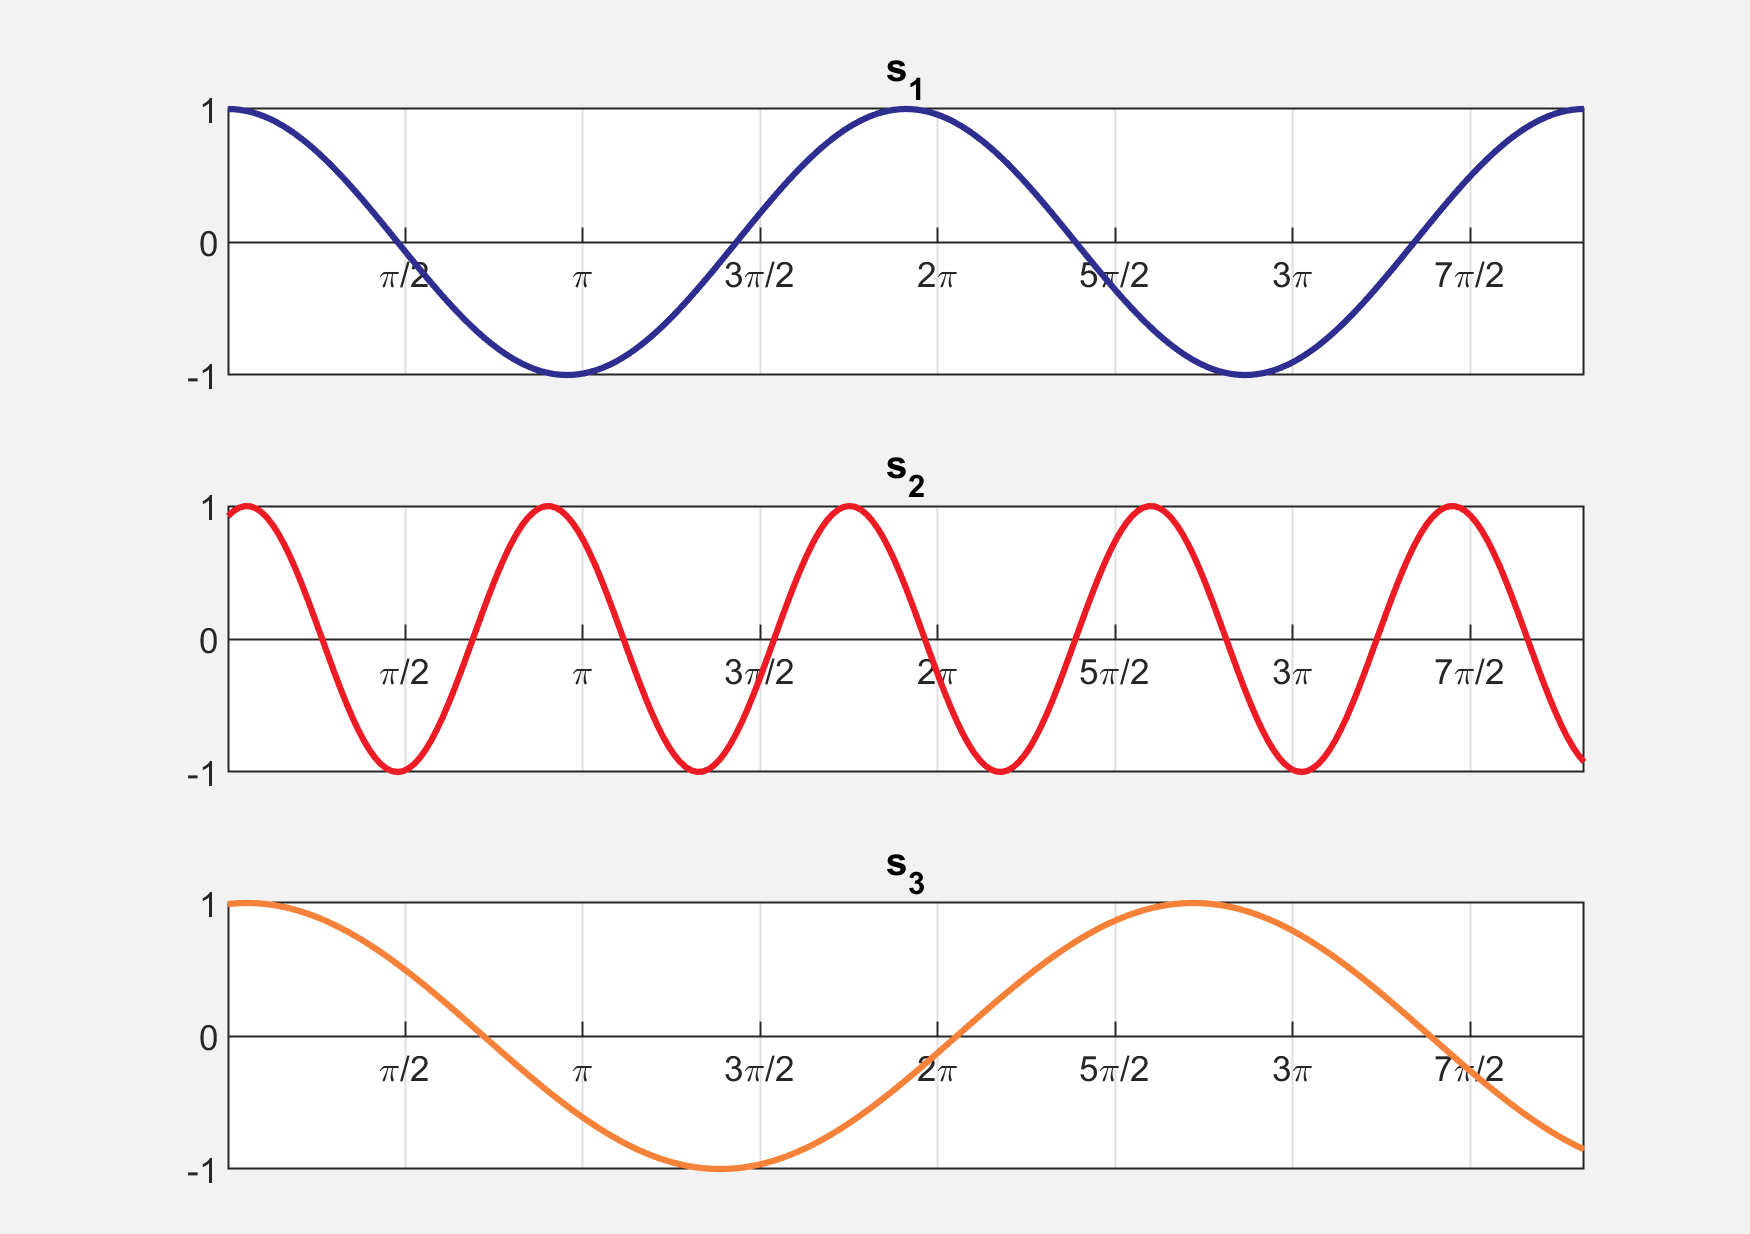
\includegraphics[width=0.9\linewidth, keepaspectratio]{./assets/411a.png}}
		}
		
	\item 
		Given are the signals:
		{
			\setlength{\abovedisplayskip}{0pt}
			\setlength{\belowdisplayskip}{6pt}
			\setlength{\abovedisplayshortskip}{0pt}
			\setlength{\belowdisplayshortskip}{0pt}
			\begin{align*}
				s_1(t) = \cos\left[{\omega_x\cdot\left(t-\tau_x\right)+\theta_x}\right] \\
				s_2(t) = \sin\left[{\omega_y\cdot\left(t-\tau_y\right)+\theta_y}\right]
			\end{align*}
		}
		and the parameters:
		
		\begin{nscenter}
			\begin{tabular}{c|lll|lll}
				& $\omega_x$ & $\tau_x$ & $\theta_x$ & $\omega_y$ & $\tau_y$ & $\theta_y$ \\
				\hline
				1 & $\pi/{3}$ & $0$ & $2\pi$ & $\pi/3$ & $1$ & $-7\pi/6$ \\
				2 & $3\pi/4$ & $1/2$ & $\pi/4$ & $11\pi/4$ & $1$ & $3\pi/8$ \\
				3 & $3/4$ & $1/2$ & $1/4$ & $3/4$ & $1$ & $13/8$ \\
			\end{tabular}
		\end{nscenter}\\
		This gives us the functions:
		{
			\setlength{\abovedisplayskip}{0pt}
			\setlength{\belowdisplayskip}{6pt}
			\setlength{\abovedisplayshortskip}{0pt}
			\setlength{\belowdisplayshortskip}{0pt}
			\begin{align*}
				s_{11}(t) = \cos\left[\frac{\pi}{3}\cdot\left(t-0\right)+2\pi\right] & \qquad 
				s_{21}(t) = \sin\left[\frac{\pi}{3}\cdot\left(t-1\right)-\frac{7\pi}{6}\right] \\
				%
				s_{12}(t) = \cos\left[\frac{3\pi}{4}\cdot\left(t-\frac{1}{2}\right)+\frac{\pi}{4}\right] & \qquad 
				s_{22}(t) = \sin\left[\frac{11\pi}{4}\cdot\left(t-1\right)+\frac{3\pi}{8}\right] \\
				%
				s_{13}(t) = \cos\left[\frac{3}{4}\cdot\left(t-\frac{1}{2}\right)+\frac{1}{4}\right] & \qquad 
				s_{23}(t) = \sin\left[\frac{3}{4}\cdot\left(t-1\right)+\frac{13}{8}\right]
			\end{align*}
		}
		\subsubsection{Solution}
		It is to be checked for which of the given combinations $s_{1i}(t)$ is identical to $s_{2i}(t)$. \\
		Since sine and cosine have a phase shift of $\SI{90}{\degree}$ ($\pi/2$) to each other, a cosine function can be converted into a sine function by adding this shift. \vspace{2pt}
		{
			\setlength{\abovedisplayskip}{0pt}
			\setlength{\belowdisplayskip}{6pt}
			\setlength{\abovedisplayshortskip}{0pt}
			\setlength{\belowdisplayshortskip}{0pt}
			
			\underline{Signal combination 1:}
			
			\begin{minipage}[t]{0.499999\linewidth}
				\begin{flalign*}
					s_{11}(t) & = \cos\left[\frac{\pi}{3}\cdot\left(t-0\right)+2\pi\right] & \\
					&=\cos\left(\frac{\pi}{3}t\right) & \\
					&=\sin\left(\frac{\pi}{3}t + \frac{\pi}{2}\right) &
				\end{flalign*}
			\end{minipage}
			\begin{minipage}[t]{0.499999\linewidth}
				\begin{flalign*}
					s_{21}(t) & = \sin\left[\frac{\pi}{3}\cdot\left(t-1\right)-\frac{7\pi}{6}\right] & \\
					&=\sin\left(\frac{\pi}{3}t - \frac{\pi}{3} - \frac{\pi}{3}\right) & \\
					&=\sin\left(\frac{\pi}{3}t - \frac{2\pi}{3}\right) &
				\end{flalign*}
			\end{minipage}
			\vspace{2pt} \\
			$\Rightarrow$ The signals have the same frequency of $\pi/3$ and amplitude of $1$, but a phase shift to each other of $\SI{30}{\degree}$, $\pi/6$ (shift on the x-axis).
			
			\vspace{4pt}
			\clearpage
			\underline{Signal combination 2:}
			
			\begin{minipage}[t]{0.499999\linewidth}
				\begin{flalign*}
					s_{12}(t) & = \cos\left[\frac{3\pi}{4}\cdot\left(t-\frac{1}{2}\right)+\frac{\pi}{4}\right] & \\
					&=\cos\left(\frac{3\pi}{4}t - \frac{3\pi}{8} + \frac{\pi}{4} \right) & \\
					&=\cos\left(\frac{3\pi}{4}t - \frac{\pi}{8}\right) & \\
					&=\sin\left(\frac{3\pi}{4}t - \frac{\pi}{8} + \frac{\pi}{2}\right) & \\
					&=\sin\left(\frac{3\pi}{4}t + \frac{3\pi}{8}\right) &
				\end{flalign*}
			\end{minipage}
			\begin{minipage}[t]{0.499999\linewidth}
				\begin{flalign*}
					s_{22}(t) & = \sin\left[\frac{11\pi}{4}\cdot\left(t-1\right)+\frac{3\pi}{8}\right] & \\
					&=\sin\left(\frac{11\pi}{4}t - \frac{11\pi}{4}+\frac{3\pi}{8}\right) & \\
					&=\sin\left(\frac{11\pi}{4}t - \frac{19\pi}{8}\right) &
				\end{flalign*}
			\end{minipage}
			\vspace{2pt} \\
			$\Rightarrow$ The signals only have the same amplitude.	
			
			\vspace{4pt}
			\underline{Signal combination 3:}
			
			\begin{minipage}[t]{0.499999\linewidth}
				\begin{flalign*}
					s_{13}(t) & = \cos\left[\frac{3}{4}\cdot\left(t-\frac{1}{2}\right)+\frac{1}{4}\right] & \\
					&=\cos\left(\frac{3\pi}{4}t - \frac{3}{8} + \frac{1}{4}\right) & \\
					&=\cos\left(\frac{3\pi}{4}t - \frac{1}{8}\right) & \\
					&=\sin\left(\frac{\pi}{3}t - \frac{1}{8} + \frac{\pi}{2}\right) &
				\end{flalign*}
			\end{minipage}
			\begin{minipage}[t]{0.5\linewidth}
				\begin{flalign*}
					s_{23}(t) & = \sin\left[\frac{3}{4}\cdot\left(t-1\right)+\frac{13}{8}\right] & \\
					&=\sin\left(\frac{3}{4}t - \frac{3}{4} + \frac{13}{8}\right) & \\
					&=\sin\left(\frac{\pi}{3}t + \frac{7}{8}\right) &
				\end{flalign*}
			\end{minipage}
			\vspace{2pt} \\
			$\Rightarrow$ As in the first combination, these two signals are also identical in terms of frequency and amplitude. However, they have a phase shift of $\SI{2,33}{\radian}$ in relation to each other.
		}
		
		\subsubsection{Matlab}
		\lstinputlisting[language=Matlab]{./assets/Lab1_411b.m}
		Signal curves\newline
		{
			\setlength{\fboxsep}{0pt}%  
			\colorbox{backcolor}{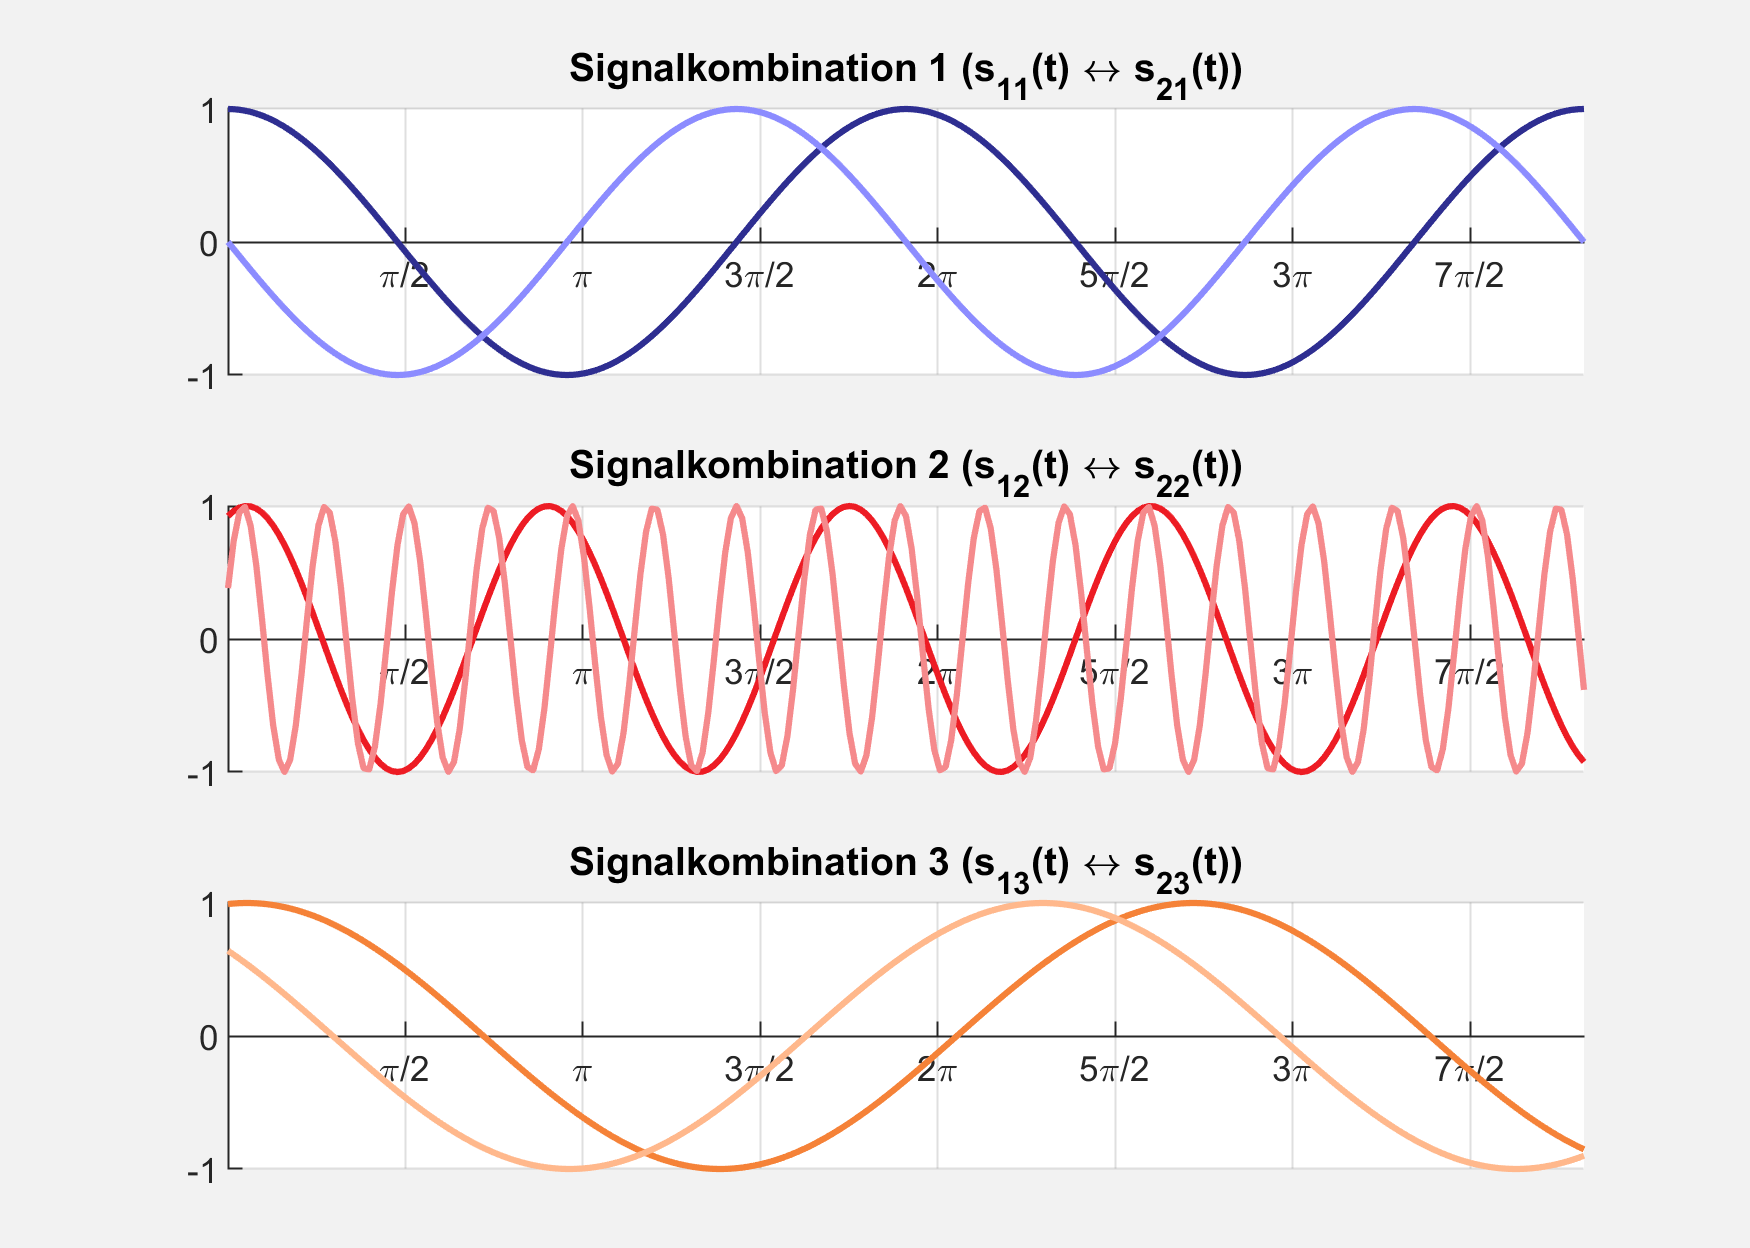
\includegraphics[width=\linewidth, keepaspectratio]{./assets/411b.png}}
		}
\end{enumerate}
\clearpage